\chapter{Arhitektura i dizajn sustava}

Arhitektura se može podijeliti na tri podsustava:

\begin{packed_item}
	\item Web poslužitelj
	\item Web aplikacija
	\item Baza podataka
\end{packed_item}

\begin{figure}[H]
	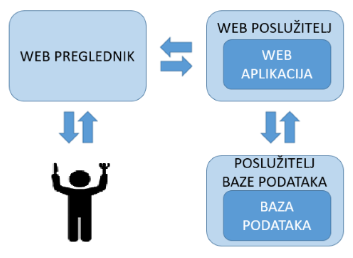
\includegraphics[scale=0.8]{slike/Slika11.png} %veličina slike u odnosu na originalnu datoteku i pozicija slike
	\centering
	\caption{Arhitektura sustava}
	\label{fig:promjene}
\end{figure}

\underline{Web preglednik} je program koji korisniku omogućuje pregled web-stranica i multimedijalnih sadržaja
vezanih uz njih. Svaki internetski preglednik je prevoditelj. Dakle, stranica je pisana u kodu koji
preglednik nakon toga interpretira kao nešto svakome razumljivo. Korisnik putem web preglednika šalje
zahtjev web poslužitelju.
\newline \underline{Web poslužitelj} osnova je rada web aplikacije. Njegova primarna zadaća je komunikacija klijenta s aplikacijom.
Komunikacija se odvija preko HTTP (engl. Hyper Text Transfer Protocol) protokola, što je protokol u prijenosu
informacija na webu. Poslužitelj je onaj koji pokreće web aplikaciju te joj prosljeđuje zahtjev. \newline Korisnik koristi
\underline{web aplikaciju} za obrađivanje željenih zahtjeva. Web aplikacija obrađuje zahtjev te ovisno o zahtjevu, pristupa
bazi podataka nakon čega preko poslužitelja vraća korisniku odgovor u obliku HTML dokumenta vidljivog u web pregledniku. \newline
\newline Programski jezik kojeg smo odabrali za izradu naše web aplikacije je Java zajedno sa Spring Boot radnim okvirom. Odabrano razvojno okruženje je Visual Studio Code.
Arhitektura sustava temeljiti će se na MVC (Model-View-Controller) konceptu. \newline
Karakteristika MVC koncepta je nezavisan razvoj pojedinih dijelova aplikacije što za posljedicu ima jednostavnije
ispitivanje kao i jednostavno razvijanje i dodavanje novih svojstava u sustav.\newline MVC koncept sastoji se od:
\begin{packed_item}
	\item \textbf{Model} - Središnja komponenta sustava. Predstavlja dinamičke strukture podataka, neovisne
	o korisničkom sučelju. Izravno upravlja podacima, logikom i pravilima aplikacije. Također prima ulazne podatke od Controllera.
	\item \textbf{View} - Bilo kakav prikaz podataka, poput grafa. Mogući su različiti prikazi iste informacije poput
	grafičkog ili tabličnog prikaza podataka.
	\item \textbf{Controller} - Prima ulaze i prilagođava ih za prosljeđivanje Modelu ili Viewu. Upravlja
	korisničkim zahtjevima i temeljem njih izvodi daljnju interakciju s ostalim elementima sustava.
\end{packed_item}

\newpage



\section{Baza podataka}

Za potrebe našeg sustava koristit ćemo relacijsku bazu podataka koja svojom strukturom olakšava modeliranje stvarnog svijeta. Gradivna jedinka baze je relacija,
odnosno tablica koja je definirana svojim imenom i skupom atributa. Zadaća baze podataka je brza i jednostavna
pohrana, izmjena i dohvat podataka za daljnju obradu. Baza podataka ove aplikacije sastoji se od sljedećih entiteta:

\begin{packed_item}
	\item Users
	\item Roles
	\item Images
	\item Ingredients
	\item Recipes
	\item Ratings
	\item \texttt{Recipe\_steps}

\end{packed_item}

\subsection{Opis tablica}

\textbf{Users}  Ovaj entitet sadržava sve važne informacije o korisniku aplikacije.
Sadrži atribute: \texttt{first\_name}, \texttt{last\_name}, \texttt{date\_of\_birth}, \texttt{email}, \texttt{id}, \texttt{password\_hash}, \texttt{username} \texttt{role\_id}. Ovaj entitet u vezi
je \textit{Many-to-One} s entitetom Roles preko atributa \texttt{role\_id}, u vezi \textit{One-to-Many}
s entitetom Recipes preko atributa \texttt{created\_by} te je u vezi \textit{One-to-Many} s entitetom Ratings
preko atributa \texttt{user\_id}.

\begin{longtblr}[
	label=none,
	entry=none
	]{
	width = \textwidth,
	colspec={|X[7,l]|X[6, l]|X[20, l]|},
	rowhead = 1,
	} %definicija širine tablice, širine stupaca, poravnanje i broja redaka naslova tablice
	\hline \multicolumn{3}{|c|}{\textbf{Users}}	 \\ \hline[3pt]
	\SetCell{LightGreen} \texttt{id} & SERIAL	&  	jedinstveni identifikator korisnika  	\\ \hline
	\texttt{first\_name}	& VARCHAR &  ime korisnika 	\\ \hline
	\texttt{last\_name} & VARCHAR & prezime korisnika \\ \hline
	\texttt{date\_of\_birth} & DATE	& datum rođenja korisnika 	\\ \hline
	\texttt{email} & VARCHAR	& korisnikov email 	\\ \hline
	\texttt{password\_hash} & VARCHAR	& korisnikova lozinka 	\\ \hline
	\texttt{username} & VARCHAR	& korisničko ime 	\\ \hline
	\SetCell{LightBlue} \texttt{role\_id}	& INT & strani ključ na entitet Roles	\\ \hline
\end{longtblr}

\newpage

\textbf{Recipes}  Ovaj entitet sadržava sve važne informacije o receptu unutar aplikacije.
Sadrži atribute: \texttt{id}, \texttt{popularity}, \texttt{title}, \texttt{created\_at},
\texttt{last\_updated\_at}, \texttt{recipe\_description}, \texttt{estimated\_time} i \texttt{created\_by}.
Ovaj entitet u vezi je \textit{One-to-Many} s entitetom Ingredients preko atributa \texttt{recipe\_id},
u vezi \textit{One-to-Many} s entitetom Images preko atributa \texttt{recipe\_id}, u vezi \textit{Many-to-One}
s entitetom Users preko atributa \texttt{created\_by}, u vezi \textit{One-to-Many} s entitetom Ratings preko atributa
\texttt{recipe\_id} te je u vezi \textit{One-to-Many} s entitetom \texttt{Recipe\_steps} preko atributa
\texttt{recipe\_id}.

\begin{longtblr}[
	label=none,
	entry=none
	]{
	width = \textwidth,
	colspec={|X[10,l]|X[6, l]|X[20, l]|},
	rowhead = 1,
	} %definicija širine tablice, širine stupaca, poravnanje i broja redaka naslova tablice
	\hline \multicolumn{3}{|c|}{\textbf{Recipes}}	 \\ \hline[3pt]
	\SetCell{LightGreen} \texttt{id} & SERIAL	&  	jedinstveni identifikator recepta  	\\ \hline
	\texttt{popularity}	& INT &  popularnost recepta 	\\ \hline
	\texttt{title} & VARCHAR & naslov recepta \\ \hline
	\texttt{created\_at} & TIMESTAMP	& datum nastanka recepta 	\\ \hline
	\texttt{last\_updated\_at} & TIMESTAMP	& datum zadnje izmjene recepta 	\\ \hline
	\texttt{recipe\_description} & VARCHAR	& kratki opis recepta 	\\ \hline
	\texttt{estimated\_time} & INT	& procijenjeno vrijeme za pripremu  	\\ \hline
	\SetCell{LightBlue} \texttt{created\_by}	& INT & strani ključ na entitet Users	\\ \hline
\end{longtblr}

\textbf{Ingredients}  Ovaj entitet predstavlja jedan sastojak unutar nekog recepta.
Sadrži atribute: \texttt{id}, \texttt{ingredient\_name}, \texttt{ingredient\_measure},
\texttt{ingredient\_quantity} i \texttt{ingredient\_order}.
Ovaj entitet u vezi je \textit{Many-to-One} s entitetom Recipes preko atributa \texttt{recipe\_id}.

\begin{longtblr}[
	label=none,
	entry=none
	]{
	width = \textwidth,
	colspec={|X[11,l]|X[6, l]|X[20, l]|},
	rowhead = 1,
	} %definicija širine tablice, širine stupaca, poravnanje i broja redaka naslova tablice
	\hline \multicolumn{3}{|c|}{\textbf{Ingredients}}	 \\ \hline[3pt]
	\SetCell{LightGreen} \texttt{id} & SERIAL	&  	jedinstveni identifikator sastojka  	\\ \hline
	\texttt{ingredient\_name}	& VARCHAR &  ime sastojka 	\\ \hline
	\texttt{ingredient\_quantity} & INT & količina sastojka \\ \hline
	\texttt{ingredient\_measure} & VARCHAR	& ime mjere sastojka(ml, g, kg) 	\\ \hline
	\texttt{ingredient\_order} & INT	& redni broj sastojka unutar recepta  	\\ \hline
	\SetCell{LightBlue} \texttt{recipe\_id}	& INT & strani ključ na entitet Recipes	\\ \hline
\end{longtblr}

\textbf{Ratings}  Ovaj entitet predstavlja ocjenu na određeni recept.
Sadrži atribute: \texttt{id}, \texttt{rating\_value}, \texttt{user\_id} i \texttt{recipe\_id}.
Ovaj entitet u vezi je \textit{Many-to-One} s entitetom Recipes preko atributa \texttt{recipe\_id}
te je u vezi \textit{Many-to-One} s entitetom Users preko atributa \texttt{user\_id}

\begin{longtblr}[
	label=none,
	entry=none
	]{
	width = \textwidth,
	colspec={|X[10,l]|X[6, l]|X[20, l]|},
	rowhead = 1,
	} %definicija širine tablice, širine stupaca, poravnanje i broja redaka naslova tablice
	\hline \multicolumn{3}{|c|}{\textbf{Ratings}}	 \\ \hline[3pt]
	\SetCell{LightGreen} \texttt{id} & SERIAL	&  	jedinstveni identifikator ocjene  	\\ \hline
	\texttt{rating\_value}	& INT &  vrijednost ocjene 	\\ \hline
	\SetCell{LightBlue} \texttt{user\_id}	& INT & strani ključ na entitet Users	\\ \hline
	\SetCell{LightBlue} \texttt{recipe\_id}	& INT & strani ključ na entitet Recipes	\\ \hline
\end{longtblr}

\textbf{Images}  Ovaj entitet predstavlja jednu sliku koja se dodaje prilikom dodavanja recepta.
Sadrži atribute: \texttt{id}, \texttt{image\_data}, \texttt{image\_order} i \texttt{recipe\_id}.
Ovaj entitet u vezi je \textit{Many-to-One} s entitetom Recipes preko atributa \texttt{recipe\_id}.

\begin{longtblr}[
	label=none,
	entry=none
	]{
	width = \textwidth,
	colspec={|X[10,l]|X[6, l]|X[20, l]|},
	rowhead = 1,
	} %definicija širine tablice, širine stupaca, poravnanje i broja redaka naslova tablice
	\hline \multicolumn{3}{|c|}{\textbf{Images}}	 \\ \hline[3pt]
	\SetCell{LightGreen} \texttt{id} & SERIAL	&  	jedinstveni identifikator slike  	\\ \hline
	\texttt{image\_data}	& BYTEA &  prostor koji zauzima slika u memoriji 	\\ \hline
	\texttt{image\_order}	& INT &  poredak slike prilikom dodavanja 	\\ \hline
	\SetCell{LightBlue} \texttt{recipe\_id}	& INT & strani ključ na entitet Recipes	\\ \hline
\end{longtblr}

\textbf{\texttt{Recipe\_steps}}  Ovaj entitet predstavlja jedan korak pripreme u receptu.
Sadrži atribute: \texttt{id}, \texttt{step\_order}, \texttt{step\_description} i \texttt{recipe\_id}.
Ovaj entitet u vezi je \textit{Many-to-One} s entitetom Recipes preko atributa \texttt{recipe\_id}.

\begin{longtblr}[
	label=none,
	entry=none
	]{
	width = \textwidth,
	colspec={|X[10,l]|X[6, l]|X[20, l]|},
	rowhead = 1,
	} %definicija širine tablice, širine stupaca, poravnanje i broja redaka naslova tablice
	\hline \multicolumn{3}{|c|}{\textbf{\texttt{Recipe\_steps}}}	 \\ \hline[3pt]
	\SetCell{LightGreen} \texttt{id} & SERIAL	&  	jedinstveni identifikator koraka pripreme  	\\ \hline
	\texttt{step\_order}	& INT &  redni broj koraka pripreme 	\\ \hline
	\texttt{step\_description}	& VARCHAR &  kratki opis koraka pripreme 	\\ \hline
	\SetCell{LightBlue} \texttt{recipe\_id}	& INT & strani ključ na entitet Recipes	\\ \hline
\end{longtblr}

\textbf{Roles}  Ovaj entitet predstavlja ulogu korisnika u sustavu.
Sadrži atribute: \texttt{id} i \texttt{role\_name}.
Ovaj entitet u vezi je \textit{One-to-Many} s entitetom Users preko atributa \texttt{role\_id}.

\begin{longtblr}[
	label=none,
	entry=none
	]{
	width = \textwidth,
	colspec={|X[10,l]|X[6, l]|X[20, l]|},
	rowhead = 1,
	} %definicija širine tablice, širine stupaca, poravnanje i broja redaka naslova tablice
	\hline \multicolumn{3}{|c|}{\textbf{Roles}}	 \\ \hline[3pt]
	\SetCell{LightGreen} \texttt{id} & SERIAL	&  	jedinstveni identifikator uloge  	\\ \hline
	\texttt{role\_name}	& VARCHAR &  ime uloge (korisnik, moderator) 	\\ \hline
\end{longtblr}

\newpage

\subsection{Dijagram baze podataka}


\begin{figure}[H]
	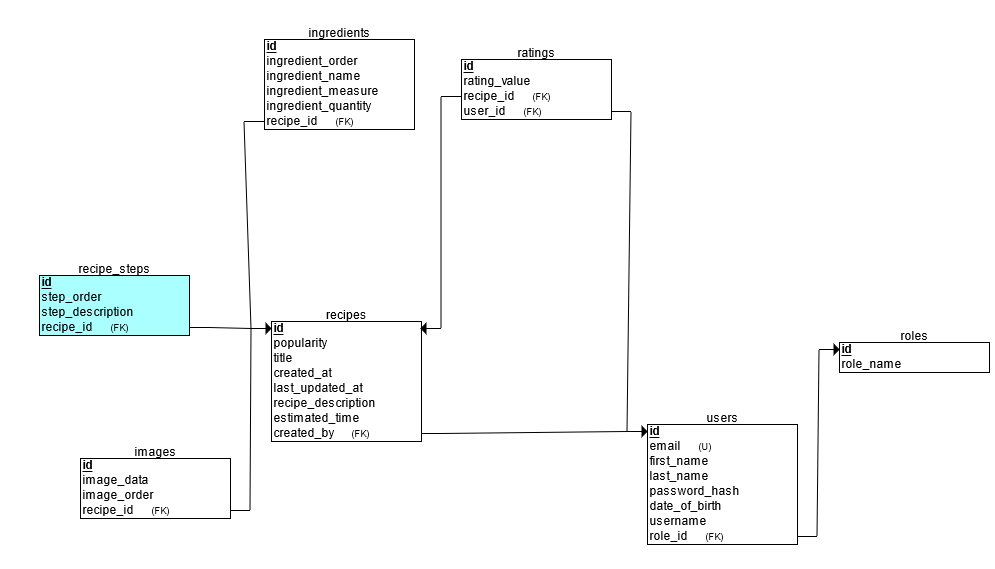
\includegraphics[scale=0.65]{slike/Slika12.png} %veličina slike u odnosu na originalnu datoteku i pozicija slike
	\centering
	\caption{E-R dijagram baze podataka}
	\label{fig:promjene}
\end{figure}


\eject


\section{Dijagram razreda}
Na slikama 4.3, 4.4 i 4.5 prikazani su razredi koji pripadaju backend dijelu MVC arhitekture. Razredi prikazani na 4.3 su Model razredi koji su implementacije entiteta baze. Razredi prikazani na slici 4.3 su Controller razredi te oni implementiraju funkcionalnosti u ovisnosti na HTTP upit i vraćaju valjani odgovor u JSON formatu. Bazi se pristupa preko Interfacea koji nasljeđuju JpaRepository. \\

Zbog lakše organizacije razredi su podijeljeni na tri logičke jedinice te su prikazani odvojenim dijagramima. Iz naziva i tipova atributa mogu se zaključiti ostale ovisnosti među razredima.

\begin{figure}[H]
	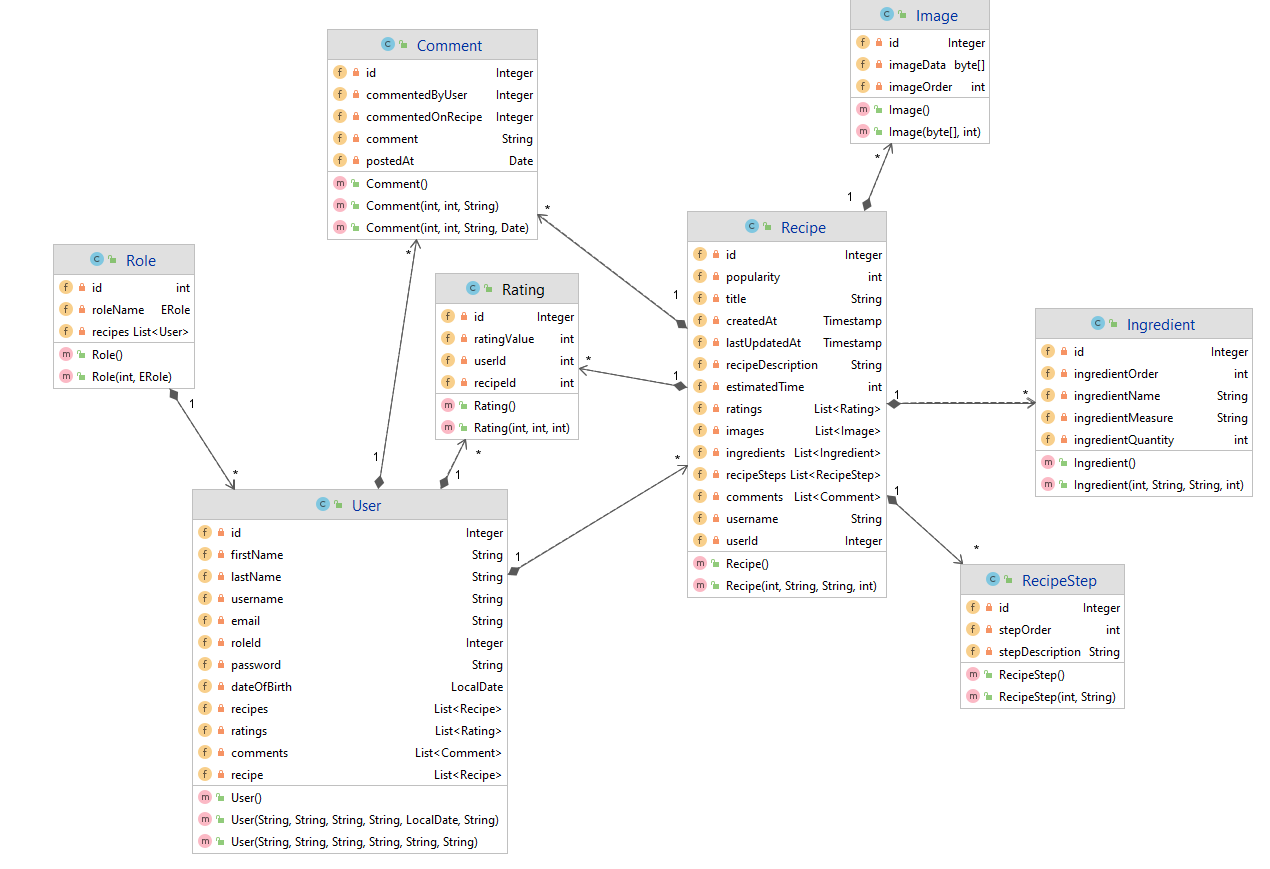
\includegraphics[scale=0.55]{slike/modelsDiagram.PNG} %veličina slike u odnosu na originalnu datoteku i pozicija slike
	\centering
	\caption{Dijagram razreda - Models}
	\label{fig:promjene}
\end{figure}

\begin{figure}[H]
	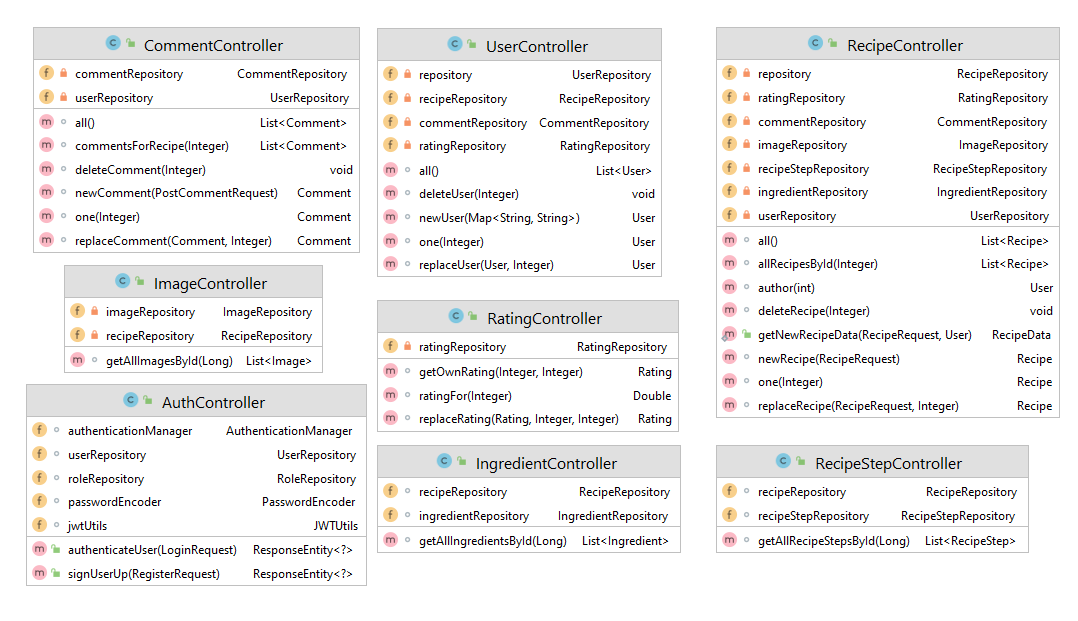
\includegraphics[scale=0.6]{slike/controllerDiagram.PNG} %veličina slike u odnosu na originalnu datoteku i pozicija slike
	\centering
	\caption{Dijagram razreda - Controllers}
	\label{fig:promjene}
\end{figure}

\begin{figure}[H]
	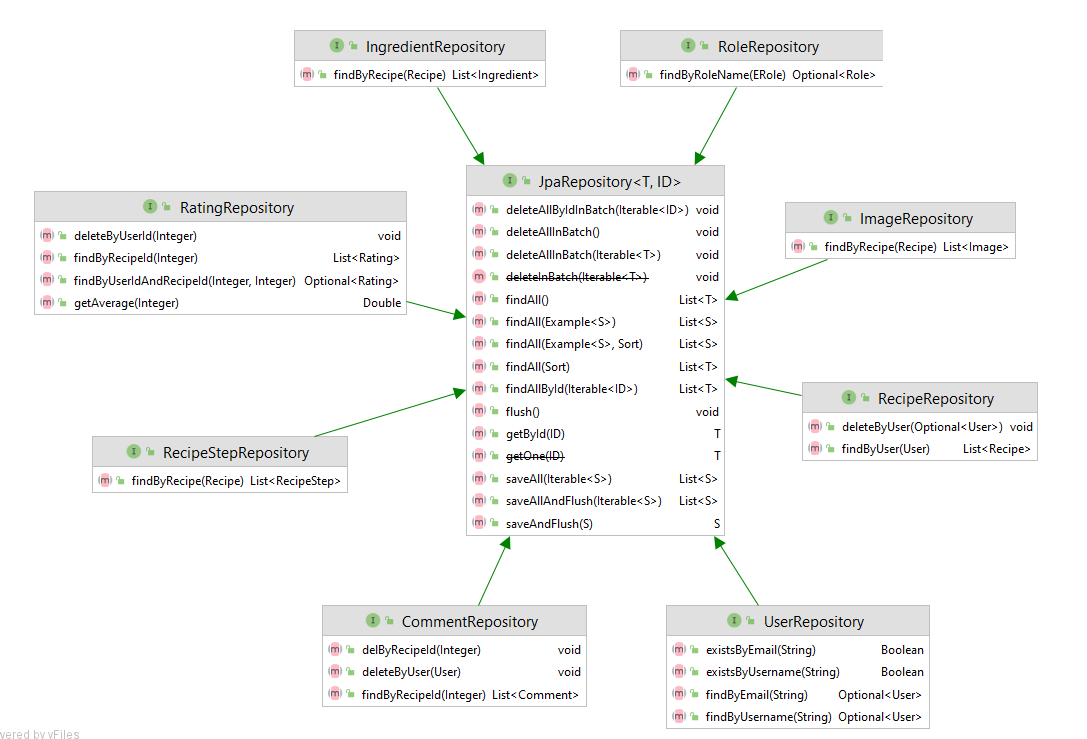
\includegraphics[scale=0.6]{slike/repositoriesDiagram.PNG} %veličina slike u odnosu na originalnu datoteku i pozicija slike
	\centering
	\caption{Dijagram razreda - Repositories}
	\label{fig:promjene}
\end{figure}


\eject

\section{Dijagram stanja}

Dijagram stanja prikazuje stanja objekta te prijelaze iz jednog stanja u drugo temeljene na događajima. Na slici 4.6 vidljiv je dijagram stanja registriranog korisnika. Korisnikove mogućnosti, osim pregleda svih recepata koji se prikazuju pri učitavanju stranice, su i pregled vlastitih recepata. Klikom na Sortiraj, korisnik može sortirati recepte po ocjeni, preporuci i popularnosti te mu je omogućen lakši pregled istih. 

Na istoj stranici, korisnik može pretražiti recepte te se tu otvaraju dvije mogućnosti, pretraživanje po sastojku te pretraživanje po imenu sve u svrhu lakšeg pretraživanja. Klijent izlistane recepte može ocijeniti, pregledati i komentirati. 
Klikom na "Moji recepti", korisniku se prikazuju svi njegovi dosadašnji recepti. Svoje recepte korisnik može obrisati, klikom na "Izbriši recept", sortirati klikom na "Sortiraj" te urediti pojedini recept.

\begin{figure}[H]
	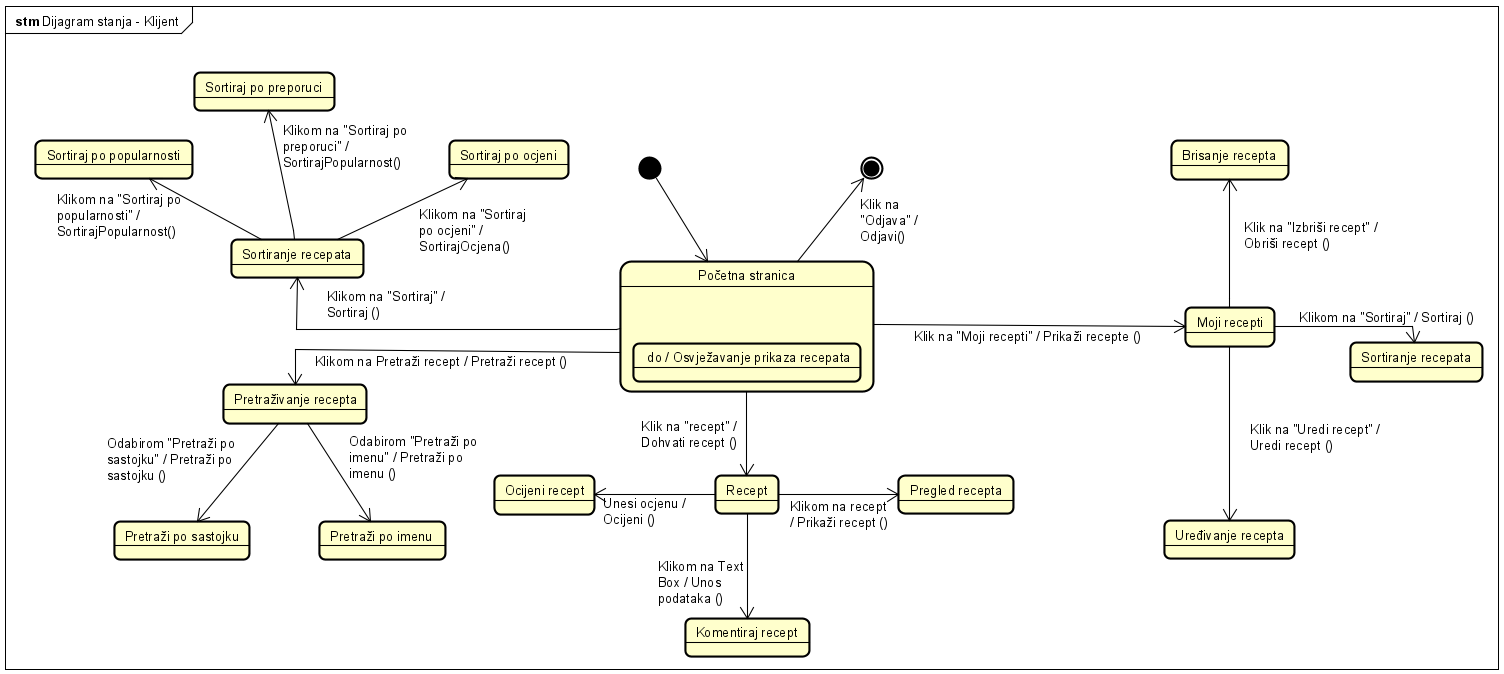
\includegraphics[scale=0.5]{slike/StateD2.PNG} %veličina slike u odnosu na originalnu datoteku i pozicija slike
	\centering
	\caption{Dijagram stanja}
	\label{fig:promjene}
\end{figure}

\eject

\section{Dijagram aktivnosti}

Dijagram aktivnosti modelira ponašanja nizom akcija. Primjenjuje se za modeliranje poslovnih procesa te upravljačkog i podatkovnog toka. Na slici 4.7 prikazan je Dijagram aktivnosti za unos novog recepta. Korisnik na početku učitava stranicu na koju nije prijavljen. Neprijavljeni korisnik i dalje ima mnoge mogućnosti ali da bi dodao svoj recept on se mora prijaviti u sustav. 

Korisnik se prijavljuje klikom na "Prijava" te se učitava stranica za prijavu. Podaci prijave se šalju Bazi podataka na validaciju te nakon njene potvrde, korisniku je omogućen daljnji pristup unosa recepta. Korisnik klikom na dodaj recept unosi podatke o receptu te pri tome mora zadovoljiti uvjete kao što su maksimalnih 5 slika koje može a i ne mora unijeti. Ujedno, potrebno je unijeti barem jedan korak pripreme te se uneseni podaci provjeravaju u Bazi podataka. Nakon zadovoljavajućeg unosa podataka recepta, šalje se poruka da je recept valjano dodan.

\begin{figure}[H]
	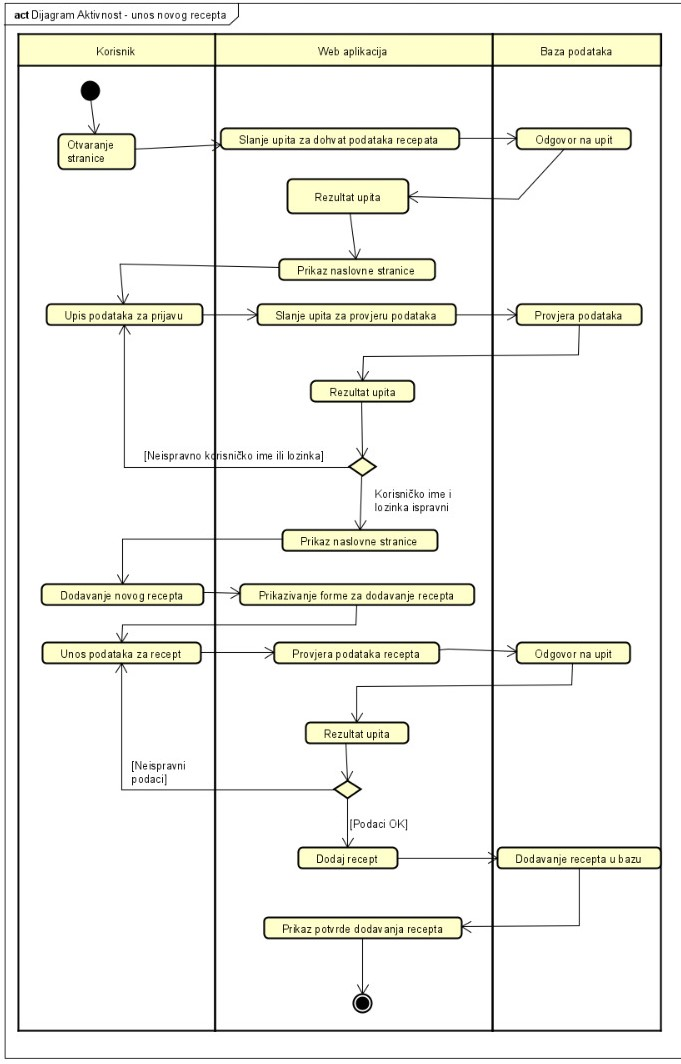
\includegraphics[scale=0.6]{slike/ActivityD.PNG} %veličina slike u odnosu na originalnu datoteku i pozicija slike
	\centering
	\caption{Dijagram aktivnosti}
	\label{fig:promjene}
\end{figure}

\eject
\section{Dijagram komponenti}

\text\noindent
Dijagram komponenti prikazan na slici 4.8 opisuje organizaciju i međusobnu ovisnost komponenti, unutrašnje strukture i odnose prema okolini.
Preko sučelja "Dohvati HTML, CSS i JS datoteke" poslužuju se datoteke za \textit{frontend} dio web aplikacije.
\textit{Frontend} dio web aplikacije se sastoji od niza TypeScript datoteka koje predstavljaju aktore koji tim datotekama mogu pristupiti.
Preko sučelja "Dohvati JSON" pristupa se REST API komponenti. REST API poslužuje podatke koje pripadaju \textit{backend} dijelu web apliakcije.
JPA Repository služi ya dohvaćanje tablica iz baze podataka koristeći SQL upite. 

\begin{figure}[H]
	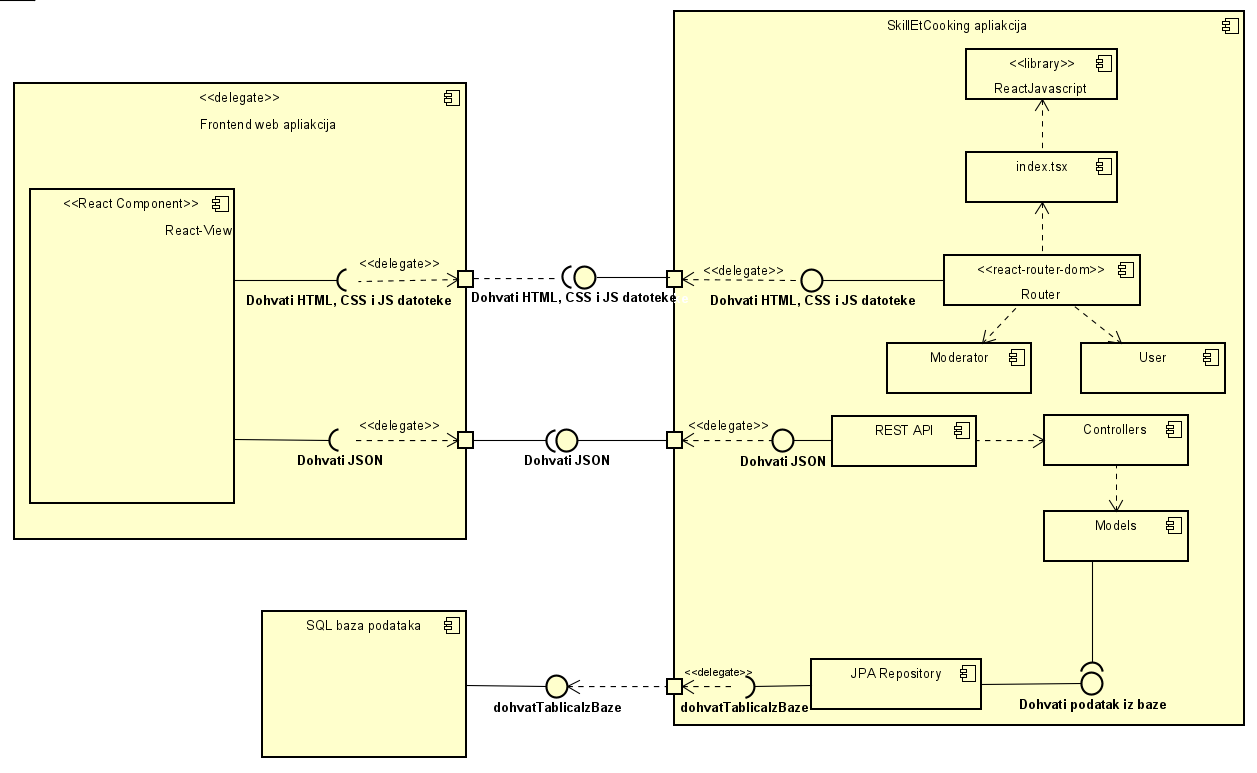
\includegraphics[scale=0.6]{slike/dijagramKomp.png} %veličina slike u odnosu na originalnu datoteku i pozicija slike
	\centering
	\caption{Dijagram komponenti}
	\label{fig:promjene}
\end{figure}